%
% Niniejszy plik stanowi przykład formatowania pracy magisterskiej na
% Wydziale MIM UW.  Szkielet użytych poleceń można wykorzystywać do
% woli, np. formatujac wlasna prace.
%
% Zawartosc merytoryczna stanowi oryginalnosiagniecie
% naukowosciowe Marcina Wolinskiego.  Wszelkie prawa zastrzeżone.
%
% Copyright (c) 2001 by Marcin Woliński <M.Wolinski@gust.org.pl>
% Poprawki spowodowane zmianami przepisów - Marcin Szczuka, 1.10.2004
% Poprawki spowodowane zmianami przepisow i ujednolicenie 
% - Seweryn Karłowicz, 05.05.2006
% Dodanie wielu autorów i tłumaczenia na angielski - Kuba Pochrybniak, 29.11.2016

% dodaj opcję [licencjacka] dla pracy licencjackiej
% dodaj opcję [en] dla wersji angielskiej (mogą być obie: [licencjacka,en])
\documentclass[licencjacka]{pracamgr}
\usepackage[polish]{babel}
\usepackage{graphicx}
\usepackage{caption}
\usepackage{subcaption}

% Dane magistranta:
\autor{Aleksander Mućk}{382184}


% Dane magistrantów:
%\autor{Aleksander Mućk}{342007}

\title{Algorytmy do klastrowania duplikacji genomowych}


\tytulang{Algorithms for the clustering of genomic duplication}

%kierunek: 
% - matematyka, informacyka, ...
% - Mathematics, Computer Science, ...
\kierunek{Bioinformatyka i Biologia Systemów}

% informatyka - nie okreslamy zakresu (opcja zakomentowana)
% matematyka - zakres moze pozostac nieokreslony,
% a jesli ma byc okreslony dla pracy mgr,
% to przyjmuje jedna z wartosci:
% {metod matematycznych w finansach}
% {metod matematycznych w ubezpieczeniach}
% {matematyki stosowanej}
% {nauczania matematyki}
% Dla pracy licencjackiej mamy natomiast
% mozliwosc wpisania takiej wartosci zakresu:
% {Jednoczesnych Studiow Ekonomiczno--Matematycznych}

% \zakres{Tu wpisac, jesli trzeba, jedna z opcji podanych wyzej}

% Praca wykonana pod kierunkiem:
% (podać tytuł/stopień imię i nazwisko opiekuna
% Instytut
% ew. Wydział ew. Uczelnia (jeżeli nie MIM UW))
\opiekun{dra hab. Pawła Góreckiego\\
  }

% miesiąc i~rok:
\date{Sierpień 2019}

%Podać dziedzinę wg klasyfikacji Socrates-Erasmus:
\dziedzina{ 
%11.0 Matematyka, Informatyka:\\ 
%11.1 Matematyka\\ 
%11.2 Statystyka\\ 
%11.3 Informatyka\\ 
%11.4 Sztuczna inteligencja\\ 
%11.5 Nauki aktuarialne\\
11.9 Inne nauki matematyczne i informatyczne
}

%Klasyfikacja tematyczna wedlug AMS (matematyka) lub ACM (informatyka)
\klasyfikacja{Computional biology, Applied computing, Life and medical sciences}

% Słowa kluczowe:
\keywords{duplikacja genu, drzewo genów, drzewo gatunków, analiza filogenetyczna, drzewo uzgadniające, Python, scenariusz ewolucyjny, strata genu, minimalizacja kosztu ewolucyjnego}

% Tu jest dobre miejsce na Twoje własne makra i~środowiska:
\newtheorem{defi}{Definicja}[section]

% koniec definicji

\begin{document}

\maketitle

%tu idzie streszczenie na strone poczatkowa

\begin{abstract}
   Niniejsza praca przedstawia propozycje rozwiązań algorytmicznych dla problemów klastrowania duplikacji genomowych w oparciu o scenariusze ewolucyjne. W części pierwszej wprowadzane są podstawowe pojęcia dotyczące drzew genów, gatunków, modeli ich uzgadniania oraz tworzenia scenariuszy ewolucyjnych. Omówiony został również problem przeliczania i klastrowania duplikacji genomowych. W części drugiej opisana została proponowana heurystyka wraz z przykładowymi testami oraz jej implementacją w języku Python.
\end{abstract}


\renewcommand{\contentsname}{Spis Treści}
\tableofcontents
%\listoffigures
%\listoftables

\chapter*{Wprowadzenie}
\addcontentsline{toc}{chapter}{Wprowadzenie}


Uzgadnianie drzew filogenetycznych jest, przez rozmiar danych i coraz bardziej skomplikowane modele, niezwykle złożone zarówno obliczeniowo jak i koncepcyjnie. Badania drzew genów i gatunków, a w szczególności zależności między nimi może odpowiedzieć na pytania w jaki sposób wyodrębniały się gatunki przez pryzmat zmian w ich genomie. Mimo wszystko jednak należy pamiętać, że pokrewieństwo gatunków nie zawsze implikuje pokrewieństwo genów, których drzewo ewolucyjne nie musi pokrywać się z drzewem zawierających je gatunków, które samo w sobie nie jest tak bardzo bardzo zróżnicowane jak drzewo genów. Tworzenie scenariuszy ewolucyjnych, dzięki którym możemy poznać w jaki sposób ewolucja genów wpływała na ewolucję gatunków jest zadaniem nietrywialnym. Potrzebne są narzędzia, które potrafiłyby ocenić scenariusze pod kątem ilości epizodów ewolucyjnych. Epizody, takie jak duplikacje genomowe, mogą być wyznacznikami prawdopodobieństwa danego scenariusza. Zagadnienie to jest jeszcze bardziej wymagające od uzgodnienia pojedynczego drzewa, ponieważ jeden scenariusz zawiera wiele drzew genów co wpływa na poziom złożoności obliczeń. W niniejszej pracy proponowany jest algorytm, który ocenia zbiór scenariuszy tworząc na ich podstawie jeden, którego koszt, liczony jako ilość duplikacji, będzie możliwie najmniejszy.
\\
Praca składa się z~czterech rozdziałów i~dodatków.
W~rozdziale \ref{r:pojecia} przedstawiono podstawowe pojęcia dotyczące drzew genów, drzew gatunków oraz modeli i scenariuszy ewolucyjnych.  
Rozdział~\ref{r:heurystyka} przedstawia propozycję heurystyki wraz~z jej testami na rzeczywistych danych.  W~rozdziale tym opisano również implementację i sposób użycia programu napisanego na podstawie przybliżonej we wcześniejszej sekcji heurystyki.
Ostatni rozdział zawiera przemyślenia dotyczące możliwego użycia algorytmu i perspektyw jego rozwoju. W~dodatkach umieszczono fragmenty kodu, przykładowe dane wejściowe i~wyniki działania algorytmu.

\chapter{Podstawowe pojęcia}\label{r:pojecia}

W tym rozdziale poruszane są pojęcia i definicje niezbędne do zrozumienia problematyki klastrowania duplikacji genomowych. 
\section{Wstęp biologiczny}

Ewolucja biologiczna jest procesem zmian w trakcie których organizmy stopniowo nabywają lub tracą pewne cechy. Jest to element kluczowy dla powstawania nowych gatunków: specjacji. Śledzenie w jaki sposób kształtowały się nowe gatunki i w jaki sposób zachodziły na Ziemi procesy ewolucyjne jest zadaniem niezwykle złożonym i wymagającym specyficznego podejścia. Jednym z możliwych sposobów przedstawienia historii ewolucyjnej gatunków jest drzewo filogenetyczne, które przedstawiają zależności ewolucyjne pomiędzy umieszczonymi na nim gatunkach lub genach. 

Początkowo za wyznacznik pokrewieństwa gatunków służyło podobieństwo morfologiczne, jednak obecnie często stosuje się metody polegające na badaniu podobieństwa danych rodzin genów. Można założyć, że im większe podobieństwo genomu danych organizmów tym bliżej są one spokrewnione. Z punktu widzenia tej pracy genom jest niczym więcej jak zbiorem genów obecnym w danym organizmie. 


\section{Drzewa genów i gatunków}

W pracy tej T niech będzie ukorzenionym, binarnym drzewem o zbiorze krawędzi $E_T$~i zbiorze węzłów~$V_T$: 
\begin{center}
T = <$V_T$ , $E_T$>.
\end{center}
%($v_1$ , $v_2$) takie, że $V_T$ \ni $v_x$ , $v_y$ .
$E_T$ zawiera pary węzłów ($v_x$ , $v_y$) takie, że $V_T$ $\ni$ $v_x$,$v_y$. Węzły z których nie wychodzą żadne krawędzie nazywane są liśćmi, a korzeń jest węzłem do którego nie prowadzą żadne krawędzie (nieposiadającym rodzica). Węzeł $v_x$ jest przodkiem węzła $v_y$ jeśli istnieje ścieżka skierowana z węzła $v_x$ do węzła $v_y$. Liczba krawędzi w ścieżce od węzła $v_x$ do węzła $v_y$ jest nazywana długością. Poddrzewem węzła $v_x$ jest drzewo oznaczone T($v_x$) w którym węzeł $v_x$ jest korzeniem.


\begin{defi}\label{Drzewa gatunków}
  Związki między gatunkami przedstawia się za pomocą drzewa~T, zwanego drzewem gatunków~S. W drzewie~S każdy z liści reprezentuje inny gatunek~Sp, a węzły wewnętrzne są specjacjami.
\end{defi}

\begin{defi}\label{Drzewa genów}
  Związki między genami w danej rodzinie przedstawia się za pomocą drzewa~T, zwanego drzewem genów~G. W drzewie~G każdy z liści reprezentuje przynależność danego genu do gatunku~Sp.
\end{defi}


\begin{figure}[h]
\centering
\begin{subfigure}{.5\textwidth}
  \centering
  \includegraphics[width=50mm]{./pictures/gene.png}
  \caption{Przykładowe drzewo genów G}
  \label{fig:sub2}
\end{subfigure}%
\begin{subfigure}{.5\textwidth}
  \centering
  \includegraphics[width=50mm]{./pictures/species.png}
  \caption{Przykładowe drzewo gatunków S}
  \label{fig:sub1}
\end{subfigure}%
\caption{Przykładowe drzewa T \cite{gsevol}}
\label{fig:test}
\end{figure}

\section{Uzgodnienie drzew}
Bardzo częste różnice struktury drzewa genów w stosunku do historii ewolucyjnej opisanej drzewem gatunków wymagają mapowania węzłów drzewa G na węzły znajdujące się w drzewie S. Jest to krok niezbędny by zrozumieć w jaki sposób ewolucja gatunków wpływała na strukturę ich genomów. 

\subsection{Mapowanie LCA}
Podstawowym algorytmem dla tego typu uzgodnień jest \textbf{algorytm LCA} (ang. \textit{Lowest Common Ancestor}; pl. \textit{Najniższy Wspólny Przodek}). Najniższym przodkiem węzłów $v_x$ i $v_y$ jest taki węzeł $v_{anc}$, który jest przodkiem obu węzłów i którego długość od korzenia drzewa jest największa.

\begin{figure}[h]
  \centering
  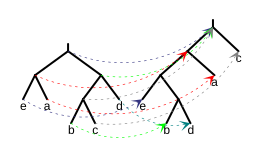
\includegraphics[width=80mm]{./pictures/mapping.png}
  \caption{Uzgodnienie LCA dla przykładowych drzew genów G i gatunków S \cite{gsevol}}
\end{figure}

\begin{defi}
Uzgodnienie drzew jest taką funkcją $MAP_{LCA}$: G $\rightarrow$ S gdzie dla każdego węzła $v_g$ z drzewa genów G przyporządkowuje się węzeł $v_s$ z drzewa gatunków S tak, że węzeł $v_s$ jest węzłem $v_{anc}$ i węzły z poddrzewa T($v_g$) są obecne w T($v_s$).
\end{defi}


\subsection{Drzewa DLS}



\section{Koszt scenariusza ewolucyjnego}


\section{Modele scenariuszy ewolucyjnych}

Podstawowy opis idei. Podział ruchów:
\\[1in]

\begin{defi}\label{TMOVE}
  TMOVE.\\[1in]
\end{defi}

\begin{defi}\label{CLOST}
  CLOST.\\[1in]
\end{defi}

\section{Opis modeli}

Dozwolone modele:
\begin{enumerate}
\item PG\\[1in]
\item FHS;\\[1in]
\end{enumerate}

\begin{figure}[tp]
  \centering
  \framebox{\vbox to 4cm{\vfil\hbox to
      7cm{\hfil\tiny.\hfil}\vfil}}
  \caption{Obrazek scenariusza}
\end{figure}

\chapter{Heurystyka}\label{r:heurystyka}

\section{Opis algorytmu}

Algorytm zakłada, że na wejściu dostępne są dane:
\begin{itemize}
\item Drzewa genów $G_1$ ... $G_k$,
\item $m_i$ scenariuszy drzewa $G_i$ opisanych jako wektory ${v_i}_1$, ${v_i}_2$ ... ${v_i}_m$ z wyliczonymi wartościami kosztu ewolucyjnego, mierzonego jako ilość duplikacji dla każdego węzła.
\end{itemize}
Istnieje wektor przybliżający rozwiązanie ME, który nazwijmy V* i który pasuje do każdego scenariusza. \\
Jednym z takich wektorów jest wektor $V_{max}$, który na każdej współrzędnej \textit{x} zawiera maksymalną wartość ${{v_i}_m}[x]$ dla każdego scenariusza \textit{m} w każdym drzewie genów $G_i$. Oczywiście nie jest to rozwiązanie najlepsze, ponieważ jest one kosztowne, ale pasuje do każdego scenariusza.

Bazując na wyliczonym wektorze $V_{max}$ heurystyka wylicza wektor V* i w pętli poprawia go w następujący sposób:
\begin{itemize}
\item Obniż jedna z wartości w wektorze V*,
\item Zaakceptuj w/w zmianę jeśli dla każdego drzewa genów istnieje scenariusz, który jest zgodny z takim wektorem epizodów,
\item Zakończ działanie jeśli nie da się poprawić żadnej współrzędnej.
\end{itemize}
Wybór współrzędnej może, zależnie od potrzeby, może być dokonywany w inny sposób:
\begin{itemize}
\item od końca wektora (od korzenia),
\item od początku (od liści),
\item losowo.
\end{itemize}


\section{Testy algorytmu}
Do sprawdzenia wyników wyliczanych przez proponowany algorytm użyty został program napisany przez dra Jarosława Paszka. Program ten korzystając z dostępnych metod algorytmicznych wylicza dokładne i najniższe możliwe wartości kosztu ewolucyjnego dla podanych modeli. \cite{rme}

\subsection{Testy algorytmu na danych rzeczywistych}
Zbiorem danych dla testu na danych rzeczywistych był zbiór Guigo zawierający 53 ukorzenione drzewa genów pochodzące od 16 eukariontów. 
\\[2in]

\subsection{Testy algorytmu na danych symulowanych}
Dane dla testów syntetycznych zostały wygenerowany w sposób losowy jednak wielkość, struktura i ilość drzew genów zostały dopasowane do zbioru Guigo. Zbiory symulowane zawierają syntetyczne drzewo gatunków z 15 etykietami oraz losowo wygenerowane 48 ukorzenione drzewa genów oparte o etykiety obecne w drzewie gatunków.

\\[2in]
\section{Dokumentacja użytkowa i~opis implementacji}\label{r:impl}
Opisana wyżej heurystyka zaimplementowana została w języku Python w wersji 3.7.4 z użyciem paradygmatu obiektowego, gdzie zbiór wszystkich scenariuszy dla wszystkich drzew, pojedynczy diagram redukcyjny otrzymany z jednego drzewa genów, a także pojedynczy scenariusz stanowią oddzielne klasy. Program pythonowy przyjmuje na wejściu listę plików w których zawarte są wyliczone scenariusze dla danego drzewa genów.
\\[1in]

Pliki przekazane do programu muszą być w określonym formacie gdzie w każdej linii dla każdego drzewa muszą znajdować się podane niżej pola w określonym porządku:
\begin{itemize}
\item id drzewa,
\item wysokość drzewa na diagramie redukcyjnym,
\item drzewo zawierające liczbę duplikacji dla danej pozycji w drzewie w porządku prefiksowym,
\item id drzew, 
\item typ zmiany w kolejności drzew.
\end{itemize}

\begin{figure}[tp]
  \centering
  \framebox{\vbox to 4cm{\vfil\hbox to
      7cm{\hfil\tiny.\hfil}\vfil}}
  \caption{Przykład pliku wejściowego}
\end{figure}


Algorytm ten, dla wygody użycia, został obudowany skryptem napisanym w języku bash, który pozwala na wyliczenie scenariuszy w modelu FHS i PG z wykorzystaniem programu DLSgen autorstwa dra hab. Pawła Góreckiego. Program ten wylicza dla danego drzewa genów i drzewa gatunków niezbędne dane w podanym powyżej formacie.

\chapter{Podsumowanie}

W~pracy przedstawiono pierwszy i dosyć intuicyjny pomysł na ocenę scenariuszy ewolucyjnych pod kątem ilości duplikacji. Należy jednak wspomnieć, że bazując samą idę da się znacząco usprawnić i zejść ze złożonością nawet do liniowej oceny, bez poprzedzającego kroku, w którym wyliczane są wszystkie scenariusze. Testy pokazują również, że opisany algorytm zwraca wyniki, które różnią się w bardzo niewielkim stopniu (o ile w ogóle) od rzeczywistego minimalnego kosztu ewolucji. 
\\[1in]

\section{Perspektywy rozwoju}


Trudno przewidzieć wszystkie możliwości rozwoju, ale te bardziej
oczywiste można wskazać już teraz.  Są to:
\begin{itemize}
\item opisy naszych algorytmów optymalizacyjnych,
\\[1in]
\item opisy naszych algorytmów optymalizacyjnych,
\\[1in]
\item opisy naszych algorytmów optymalizacyjnych,
\\[1in]
\end{itemize}

\section{Perspektywy wykorzystania}

DOPYTAĆ\\[2in]

\appendix

\chapter{Pętla programu zapisana w~języku Python wykonywana dla losowego wybierania indeksów}

\begin{verbatim}

		max_trees = []
        for scenario in self:
            all_dup_pref = [tree.duplication_prefix for tree n scenario]
            max_trees.append(self.rate_scenario(all_dup_pref))
        max_tree = self.rate_scenario(max_trees)

        if select_type == "random":

            index_list = [x for x in range(len(max_tree)) if x != 0]

            while index_list:
                index_list_position = random.randint(0, len(index_list) - 1)
                index = index_list[index_list_position]

                max_tree_temp = max_tree[:]
                max_tree_temp[index] -= 1

                for scenario in self:
                    for tree in scenario:
                        for i in range(len(tree.duplication_prefix)):
                            if max_tree_temp[i] - tree.duplication_prefix[i] < 0:
                                break
                        else:
                            break
                    else:
                        index_list.pop(index_list_position)
                        break
                else:
                    max_tree = max_tree_temp
            return max_tree, sum(max_tree)
\end{verbatim}

\chapter{Przykładowe drzewo gatunków}

\begin{center}
(prot,(fung,((chlo,embr),(arth,((acoe,anne),(echi,(chon,(oste,(amph,(moll,((mamm,(aves,rept)),agna)))))))))))
\end{center}

\begin{figure}[tp]
  \centering
  \framebox{\vbox to 4cm{\vfil\hbox to
      7cm{\hfil\tiny.\hfil}\vfil}}
  \caption{Wizualizacja drzewa gatunków}
\end{figure}

\chapter{Przykładowe drzewa genów}

{\obeylines %
(((amph,aves),mamm),chon)
((((acoe,mamm),chlo),fung),prot)
(((((echi,arth),mamm),embr),fung),prot)
}

\begin{figure}[tp]
  \centering
  \framebox{\vbox to 4cm{\vfil\hbox to
      7cm{\hfil\tiny.\hfil}\vfil}}
  \caption{Wizualizacja drzewa genów}
\end{figure}



\chapter{Przykładowy wynik działania programu
    (dla zbioru guigo)}

{\obeylines %
------------------FHS---------------------------
Data loaded. 0.0% of the data was corrupted: 0 of 53.
total random
([0, 0, 0, 0, 0, 0, 0, 0, 0, 0, 0, 0, 0, 0, 0, 0, 1, 0, 0, 0, 1, 1, 1, 1, 1, 1, 1, 1, 2, 3, 4], 18)
Done in 2.3286948204040527 .
start
([0, 0, 0, 0, 0, 0, 0, 0, 0, 0, 0, 0, 0, 0, 0, 0, 0, 0, 0, 0, 0, 0, 0, 0, 0, 0, 0, 0, 0, 0, 5], 5)
Done in 0.0676581859588623 .
end
([0, 0, 0, 0, 0, 0, 0, 0, 0, 0, 0, 0, 0, 0, 0, 0, 0, 0, 0, 0, 0, 0, 0, 0, 0, 0, 0, 1, 0, 0, 3], 4)
Done in 0.24111151695251465 .
index random
([0, 0, 0, 0, 0, 0, 0, 0, 0, 0, 0, 0, 0, 0, 0, 0, 0, 0, 0, 0, 0, 0, 0, 0, 0, 0, 0, 0, 0, 2, 3], 5)
Done in 0.0971217155456543 .
------------------PG----------------------------
Data loaded. 0.0% of the data was corrupted: 0 of 53.
total random
([0, 0, 0, 0, 0, 0, 0, 0, 0, 0, 0, 0, 0, 0, 0, 0, 0, 0, 0, 0, 0, 0, 1, 1, 0, 0, 0, 1, 1, 1, 3], 8)
Done in 0.18230891227722168 .
start
([0, 0, 0, 0, 0, 0, 0, 0, 0, 0, 0, 0, 0, 0, 0, 0, 0, 0, 0, 0, 0, 0, 1, 0, 0, 0, 0, 1, 1, 0, 3], 6)
Done in 0.006891012191772461 .
end
([0, 0, 0, 0, 0, 0, 0, 0, 0, 0, 0, 0, 0, 0, 0, 0, 0, 0, 0, 0, 0, 0, 1, 0, 0, 0, 0, 1, 1, 0, 3], 6)
Done in 0.006652355194091797 .
index random
([0, 0, 0, 0, 0, 0, 0, 0, 0, 0, 0, 0, 0, 0, 0, 0, 0, 0, 0, 0, 0, 0, 1, 0, 0, 0, 0, 1, 1, 0, 3], 6)
Done in 0.007452487945556641 .
}

\begin{thebibliography}{99}
\addcontentsline{toc}{chapter}{Bibliografia}


\bibitem[1]{gsevol} Obraz wygenerowany za pomocą serwisu http://gsevol.azor.mimuw.edu.pl 

\end{thebibliography}

\end{document}


%%% Local Variables:
%%% mode: latex
%%% TeX-master: t
%%% coding: latin-2
%%% End:
